\documentclass[14pt]{beamer}
\usepackage[T2A]{fontenc}
\usepackage[utf8]{inputenc}
\usepackage[english,russian]{babel}
\usepackage{amssymb,amsfonts,amsmath,mathtext}
\usepackage{cite,enumerate,float,indentfirst}

\graphicspath{{../images/}{images/}} 



% \usetheme[secheader]{Boadilla}
% \usecolortheme{seahorse}

\usetheme{Pittsburgh}
\usecolortheme{whale}

\beamertemplatenavigationsymbolsempty

\newcommand{\todo}{\alert}
%%% Основные сведения %%%
\newcommand{\thesisAuthor}             % Диссертация, ФИО автора
{%
    \texorpdfstring{% \texorpdfstring takes two arguments and uses the first for (La)TeX and the second for pdf
        Ладутенко Константин Сергеевич % так будет отображаться на титульном листе или в тексте, где будет использоваться переменная
    }{%
        Ладутенко, Константин Сергеевич% эта запись для свойств pdf-файла. В таком виде, если pdf будет обработан программами для сбора библиографических сведений, будет правильно представлена фамилия.
    }%
}
\newcommand{\thesisUdk}                % Диссертация, УДК
{\todo{xxx.xxx}}

\newcommand{\thesisTitleBoth}          % Диссертация, название
% {Моделирование взаимодействия оптимизированной многослойной сферы с
% плоской электромагнитной волной}
{Рассеяние и поглощение электромагнитных волн многослойными
сферическими порытиями}

\newcommand{\thesisTitle}              % Диссертация, название
{\texorpdfstring{\MakeUppercase{\thesisTitleBoth}}{\thesisTitleBoth}}

\newcommand{\thesisSpecialtyNumberBoth}    % Диссертация, специальность, номер
{01.04.05}
\newcommand{\thesisSpecialtyNumber}    % Диссертация, специальность, номер
{\texorpdfstring{\todo{\thesisSpecialtyNumberBoth}}{\thesisSpecialtyNumberBoth}}

\newcommand{\thesisSpecialtyTitleBoth}     % Диссертация, специальность, название
{Оптика}
\newcommand{\thesisSpecialtyTitle}     % Диссертация, специальность, название
{\texorpdfstring{\todo{\thesisSpecialtyTitleBoth}}{\thesisSpecialtyTitleBoth}}


% \newcommand{\thesisSpecialtyNumberBothSecond}    % Диссертация, специальность, номер
% {05.13.18}
% \newcommand{\thesisSpecialtyNumberSecond}    % Диссертация, специальность, номер
% {\texorpdfstring{\todo{\thesisSpecialtyNumberBothSecond}}{\thesisSpecialtyNumberBothSecond}}

% \newcommand{\thesisSpecialtyTitleBothSecond}     % Диссертация, специальность, название
% { Математическое моделирование, численные методы и комплексы программ}
% \newcommand{\thesisSpecialtyTitleSecond}     % Диссертация, специальность, название
% {\texorpdfstring{\todo{\thesisSpecialtyTitleBothSecond}}{\thesisSpecialtyTitleBothSecond}}



\newcommand{\thesisDegree}             % Диссертация, научная степень
{кандидата физико-математических наук}
\newcommand{\thesisCity}               % Диссертация, город защиты
{Санкт-Петербург}
\newcommand{\thesisYear}               % Диссертация, год защиты
{\todo{20XX}}
\newcommand{\thesisOrganization}       % Диссертация, организация
{Федеральное государственное автономное образовательное учреждение высшего образования <<Санкт-Петербургский национальный исследовательский университет информационных технологий, механики и оптики>>}

\newcommand{\thesisInOrganization}       % Диссертация, организация в предложном падеже: Работа выполнена в ...
{федеральном государственном автономном образовательном учреждении высшего образования <<Санкт-Петербургский национальный исследовательский университет информационных технологий, механики и оптики>>}

\newcommand{\supervisorFio}            % Научный руководитель, ФИО
{Белов Павел Александрович}
\newcommand{\supervisorRegalia}        % Научный руководитель, регалии
{\todo{доктор физико-математических наук}}

\newcommand{\opponentOneFio}           % Оппонент 1, ФИО
{\todo{Фамилия Имя Отчество}}
\newcommand{\opponentOneRegalia}       % Оппонент 1, регалии
{\todo{доктор физико-математических наук, профессор}}
\newcommand{\opponentOneJobPlace}      % Оппонент 1, место работы
{\todo{Не очень длинное название для места работы}}
\newcommand{\opponentOneJobPost}       % Оппонент 1, должность
{\todo{старший научный сотрудник}}

\newcommand{\opponentTwoFio}           % Оппонент 2, ФИО
{\todo{Фамилия Имя Отчество}}
\newcommand{\opponentTwoRegalia}       % Оппонент 2, регалии
{\todo{кандидат физико-математических наук}}
\newcommand{\opponentTwoJobPlace}      % Оппонент 2, место работы
{\todo{Основное место работы c длинным длинным длинным длинным названием}}
\newcommand{\opponentTwoJobPost}       % Оппонент 2, должность
{\todo{старший научный сотрудник}}

\newcommand{\leadingOrganizationTitle} % Ведущая организация, дополнительные строки
{\todo{Федеральное государственное бюджетное образовательное учреждение высшего профессионального образования с~длинным длинным длинным длинным названием}}

\newcommand{\defenseDate}              % Защита, дата
{\todo{DD mmmmmmmm YYYY~г.~в~XX часов}}
\newcommand{\defenseCouncilNumber}     % Защита, номер диссертационного совета
{\todo{NN}}
\newcommand{\defenseCouncilTitle}      % Защита, учреждение диссертационного совета
{\todo{Название учреждения}}
\newcommand{\defenseCouncilAddress}    % Защита, адрес учреждение диссертационного совета
{\todo{Адрес}}

\newcommand{\defenseSecretaryFio}      % Секретарь диссертационного совета, ФИО
{\todo{Фамилия Имя Отчество}}
\newcommand{\defenseSecretaryRegalia}  % Секретарь диссертационного совета, регалии
{\todo{д-р~физ.-мат. наук}}            % Для сокращений есть ГОСТы, например: ГОСТ Р 7.0.12-2011 + http://base.garant.ru/179724/#block_30000

\newcommand{\synopsisLibrary}          % Автореферат, название библиотеки
{\todo{Название библиотеки}}
\newcommand{\synopsisDate}             % Автореферат, дата рассылки
{\todo{DD mmmmmmmm YYYY года}}

\newcommand{\keywords}%                 % Ключевые слова для метаданных PDF диссертации и автореферата
{}
      % Основные сведения

\setbeamercolor{footline}{fg=blue}
\setbeamertemplate{footline}{
  \leavevmode%
  \hbox{%
  \begin{beamercolorbox}[wd=.333333\paperwidth,ht=2.25ex,dp=1ex,center]{}%
    % И. О. Фамилия, Организация кратко
    \thesisAuthorShort, \thesisOrganizationShort
  \end{beamercolorbox}%
  \begin{beamercolorbox}[wd=.333333\paperwidth,ht=2.25ex,dp=1ex,center]{}%
    % Город, 20XX
    \thesisCity, \thesisYear
  \end{beamercolorbox}%
  \begin{beamercolorbox}[wd=.333333\paperwidth,ht=2.25ex,dp=1ex,right]{}%
  Стр. \insertframenumber{} из \inserttotalframenumber \hspace*{2ex}
  \end{beamercolorbox}}%
  \vskip0pt%
}

\newcommand{\itemi}{\item[\checkmark]}

%\title{\small{Название презентации}}
\title{\small{\thesisTitle}}
\author{\small{%
\emph{Выступающий:}~\thesisAuthorShort\\%
\emph{Руководитель:}~\supervisorRegaliaShort~\supervisorFioShort}\\%
\vspace{30pt}%
\thesisOrganization%
\vspace{20pt}%
}
\date{\small{\thesisCity, \thesisYear}}

\begin{document}

\maketitle

\begin{frame}
  \frametitle{Актуальность}
  \begin{block}{\normalsize Многослойные сферические наночастицы\
      применяются для:}
    \begin{enumerate}
    \item \small лечения рака [1]
    \item медицинской диагностики [2]
    \item устройств плазмоники и нанофотоники [3-5]
    \item улучшения свойств теплоизоляторов [6]
    \item разработки солнечных элементов [7, 8]
      \item и т.д. ... 
    \end{enumerate}
  \end{block}
  \begin{minipage}{0.49\linewidth}
    \scriptsize
 [1] J. Phys. Chem. Lett. 1, 686 \textbf{(2010)}

 [2] A. Chimica Acta 469, 149 \textbf{(2002)}

 [3] AIP Adv. 3, 112111 \textbf{(2013)}

 [4] J. Appl. Phys. 116, 184508 \textbf{(2014)}

  \end{minipage}
  \begin{minipage}{0.49\linewidth}
\scriptsize
 [5] Opt. Mat. Express 3, 954 \textbf{(2013)}

 [6] Heat and Mass Transfer 58, 540 \textbf{(2013)}

 [7] Solar Energy 85, 299 \textbf{(2011)}

 [8] Opt. Express 19, 25729 \textbf{(2011)}
  \end{minipage}
\end{frame}

\begin{frame}
  \frametitle{Цель работы:}
  \begin{center}
\textbf{    Исследование рассеяния и поглощения электромагнитных волн
    многослойными сферическими наночастицами.
}  \end{center}
  \begin{center}
    \includegraphics[width=0.6\linewidth]{model3d}    \\
    % \vspace{1em}\\
  \scriptsize Рисунок из работы \textit{Ladutenko et al.}, Nanoscale, 7, 18897 (\textbf{2015})
\end{center}

\end{frame}

\begin{frame}
  \frametitle{Задачи}
  \small
  \begin{enumerate} %TODO меньше алгоритов, больше теории.
  \item Получить явные выражения для коэффициентов Ми внутри сферы.
  \item Выбрать и реализовать алгоритм оптимизации, подходящий для
    работы с произвольными параметрами модели.% , описываемой обобщённой
    % теорией Ми    
  \item Выявить основные закономерности взаимодействия с
    электромагнитной волной сферических маскирующих покрытий на
    основе диэлектриков.
  \item Исследовать эффект  вырождения мультипольных
    резонансов для сечения поглощения  света в многослойных
    сферических наночастицах.
  \end{enumerate}
  
\end{frame}

\begin{frame}
  \frametitle{Теория Ми}
  \small
  Рассеянное поле:
  \begin{align*}
{\rm  \mathbf{E}}_s &=\sum_{n=1}^{\infty} E_n \left( i a_n {\rm 
    \mathbf{N}}_{e1n}^{(3)} - b_n{\rm \mathbf{M}_{o1n}^{(3)}} \right)\\
{\rm  \mathbf{H}}_s &=\frac{k}{\omega\mu}
 \sum_{n=1}^{\infty} E_n \left( i b_n {\rm 
    \mathbf{N}}_{o1n}^{(3)} + a_n{\rm \mathbf{M}_{e1n}^{(3)}} \right)  
\end{align*}
  Поле внутри многослойной сферы:
\begin{align*}
{\rm  \mathbf{E}}_l &=\sum_{n=1}^{\infty} E_n \left(
                     c_n^{(l)}{\rm \mathbf{M}}_{o1n}^{(1)}
                     -i d_n^{(l)} {\rm  \mathbf{N}}_{e1n}^{(1)}
                     +i a_n^{(l)} {\rm  \mathbf{N}}_{e1n}^{(3)}
                     - b_n^{(l)}{\rm \mathbf{M}}_{o1n}^{(3)} 
                     \right)\label{eq:3p1}\\
{\rm  \mathbf{H}}_l &=\frac{k_l}{\omega\mu} \sum_{n=1}^{\infty} E_n
                     \left(
                      d_n^{(l)}{\rm \mathbf{M}}_{e1n}^{(1)} 
                     +i c_n^{(l)} {\rm  \mathbf{N}}_{o1n}^{(1)} 
                     -i b_n^{(l)} {\rm  \mathbf{N}}_{o1n}^{(3)} 
                     - a_n^{(l)}{\rm \mathbf{M}}_{e1n}^{(3)} 
                     \right)
\end{align*}
\end{frame}

\begin{frame}
  \frametitle{Теория Ми}
  \small
  Из граничных условий на непрерывность
нормальных компонент полей на границе между слоями (\textit{W. Yang},
Applied Optics 42, 1710 \textbf{2003}):
\begin{equation*} % \tag{S} % tag - вписывает свой текст
    % \begin{multlined}
    \begin{alignedat}{2}
d^{(l+1)}_{n}m_{l} \psi^{\prime}_{n}&{\left (m_{l+1} x_{l} \right )}
- a^{(l+1)}_{n} m_{l} \zeta^{\prime}_{n}{\left (m_{l+1} x_{l} \right )}-\\
& - d^{(l)}_{n} m_{l+1} \psi^{\prime}_{n}{\left (m_{l} x_{l} \right )} 
+ a^{(l)}_{n} m_{l+1} \zeta^{\prime}_{n}{\left (m_{l} x_{l} \right )}
= 0
\end{alignedat}
\end{equation*}
\begin{equation*} % \tag{S} % tag - вписывает свой текст
  \label{eq:A2d2}
\begin{alignedat}{2}
c^{(l+1)}_{n} m_{l} \psi_{n}&{\left (m_{l+1} x_{l} \right )}
  - b^{(l+1)}_{n} m_{l} \zeta_{n}{\left (m_{l+1} x_{l} \right )}-\\
&- c^{(l)}_{n} m_{l+1} \psi_{n}{\left (m_{l} x_{l} \right )} 
+b^{(l)}_{n} m_{l+1} \zeta_{n}{\left (m_{l} x_{l} \right )}  =0
\end{alignedat}
\end{equation*}
\begin{equation*} % \tag{S} % tag - вписывает свой текст
  \label{eq:A2d3}
\begin{alignedat}{2}
c^{(l+1)}_{n} \psi^{\prime}_{n}&{\left (m_{l+1} x_{l} \right )}
- b^{(l+1)}_{n} \zeta^{\prime}_{n}{\left (m_{l+1} x_{l} \right )}-\\
&- c^{(l)}_{n} \psi^{\prime}_{n}{\left (m_{l} x_{l} \right )} 
+b^{(l)}_{n} \zeta^{\prime}_{n}{\left (m_{l} x_{l} \right )}   =0
\end{alignedat}
\end{equation*}
\begin{equation*} % \tag{S} % tag - вписывает свой текст
\begin{alignedat}{2}
 d^{(l+1)}_{n} \psi_{n}&{\left (m_{l+1} x_{l} \right )}
- a^{(l+1)}_{n} \zeta_{n}{\left (m_{l+1} x_{l} \right )}-\\
& - d^{(l)}_{n} \psi_{n}{\left (m_{l} x_{l} \right )} 
+ a^{(l)}_{n} \zeta_{n}{\left (m_{l} x_{l} \right )}   =0
\end{alignedat}
% \end{multlined}
\end{equation*}
\end{frame}

\begin{frame}
  \frametitle{Коэффициенты Ми}
  \footnotesize
  В результате получаем (\textit{Ladutenko et al}, Comp. Phys. Comm., V.214,
  p.225, \textbf{2017}):

\begin{equation*}
\label{eq:6p1}
a^{(l)}_n = \frac
{
    {D^{(1)}_{n}}{\left (m_{l} x_{l} \right )}
    T_1\left (m_{l+1} x_{l} \right )
    +
    T_3\left (m_{l+1} x_{l} \right )
    m_{l}/m_{l+1}
}
{
   \zeta_{n}\left (m_{l} x_{l} \right )
   U\left (m_{l} x_{l} \right )
}
\end{equation*}
\begin{equation*}
\label{eq:6p2}
b^{(l)}_n = \frac
{
    {D^{(1)}_{n}}{\left (m_{l} x_{l} \right )}
    T_2\left (m_{l+1} x_{l} \right )
    m_{l}/m_{l+1}
    +
    T_4\left (m_{l+1} x_{l} \right )
}
{
   \zeta_{n}\left (m_{l} x_{l} \right )
   U\left (m_{l} x_{l} \right )
}
\end{equation*}
\begin{equation*}
\label{eq:6p3}
c^{(l)}_n = \frac
{
    {D^{(3)}_{n}}{\left (m_{l} x_{l} \right )}
    T_2\left (m_{l+1} x_{l} \right )
    m_{l}/m_{l+1}
    +
    T_4\left (m_{l+1} x_{l} \right )
}
{
   \psi_{n}\left (m_{l} x_{l} \right )
   U\left (m_{l} x_{l} \right )
}
\end{equation*}
\begin{equation*}
\label{eq:6p4}
d^{(l)}_n = \frac
{
    {D^{(3)}_{n}}{\left (m_{l} x_{l} \right )}
    T_1\left (m_{l+1} x_{l} \right )
    +
    T_3\left (m_{l+1} x_{l} \right )
    m_{l}/m_{l+1}
}
{
   \psi_{n}\left (m_{l} x_{l} \right )
   U\left (m_{l} x_{l} \right )
}
\end{equation*}
  \scriptsize
  \begin{minipage}{0.4\linewidth}
\begin{equation*}
  T_1(z) =   a^{(l+1)}_{n}  \zeta_{n}(z) 
           - d^{(l+1)}_{n}  \psi_{n}(z)\:,\qquad
\end{equation*}
\begin{equation*}
  T_2(z) =   b^{(l+1)}_{n}  \zeta_{n}(z) 
           - c^{(l+1)}_{n}  \psi_{n}(z)\:,\qquad
\end{equation*}
\end{minipage}
\begin{minipage}{0.49\linewidth}
\begin{equation*}
  T_3(z) =  d^{(l+1)}_{n}  D^{(1)}_{n}(z)  \psi_{n}(z) 
          - a^{(l+1)}_{n}  D^{(3)}_{n}(z)  \zeta_{n} (z)\:,
\end{equation*}
\begin{equation*}
  T_4(z) =  c^{(l+1)}_{n}  D^{(1)}_{n}(z)  \psi_{n}(z) 
          - b^{(l+1)}_{n}  D^{(3)}_{n}(z)  \zeta_{n} (z)\:,
\end{equation*}
\end{minipage}
  \begin{equation*}
  U(z) =    {D^{(1)}_{n}}(z) - {D^{(3)}_{n}}(z)\:,\quad
 D^{(1)}_{n} = \psi^{\prime}_{n}/\psi_{n}\:,\quad
D^{(3)}_{n} = \zeta^{\prime}_{n}/\zeta_{n}
\end{equation*}
\end{frame}

\begin{frame}
  \frametitle{Положение 1}
  \begin{center}
    В задаче рассеяния плоской волны на многослойной сфере
    коэффициенты Ми внутри сферы могут быть явно выражены в виде
    обратной рекуррентной последовательности через логарифмические
    производные функций Риккати-Бесселя.
  \end{center}
\end{frame}

\begin{frame} {\normalsize Разработка новых дизайнов многослойных
    наночастиц}
  \small \underline{\textit{Дизайн}} сферической наночастицы --- радиусы и показатели преломлений
  составных слоёв.


  \vspace{1em}
  \normalsize
  \textbf{Стохастическая оптимизация}
  \small
    \begin{enumerate}
    \item Вначале создаются несколько дизайнов, у которых показатель
      преломления и толщина каждого слоя выбирается случайным образом.
    \item При помощи некого набора правил эти дизайны итеративно
      \textit{\textbf{улучшаются}}.
    \end{enumerate}

  В работе был реализован алгоритм адаптивной дифференциальной
  эволюции  JADE+:
    \begin{itemize}
    \item J. Zhang and A. Sanderson, Evolutionary Computation, IEEE
    Transactions on 13, 945 (2009).
  \item \textbf{https://github.com/kostyfisik/jade}
    \end{itemize}

\end{frame}

\begin{frame}
  \frametitle{Маскирующее покрытие:}
%   \begin{center}
% \textbf{    Исследование рассеяния и поглощения электромагнитных волн
%     многослойными сферическими наночастицами.
% }  \end{center}
  \begin{center}
    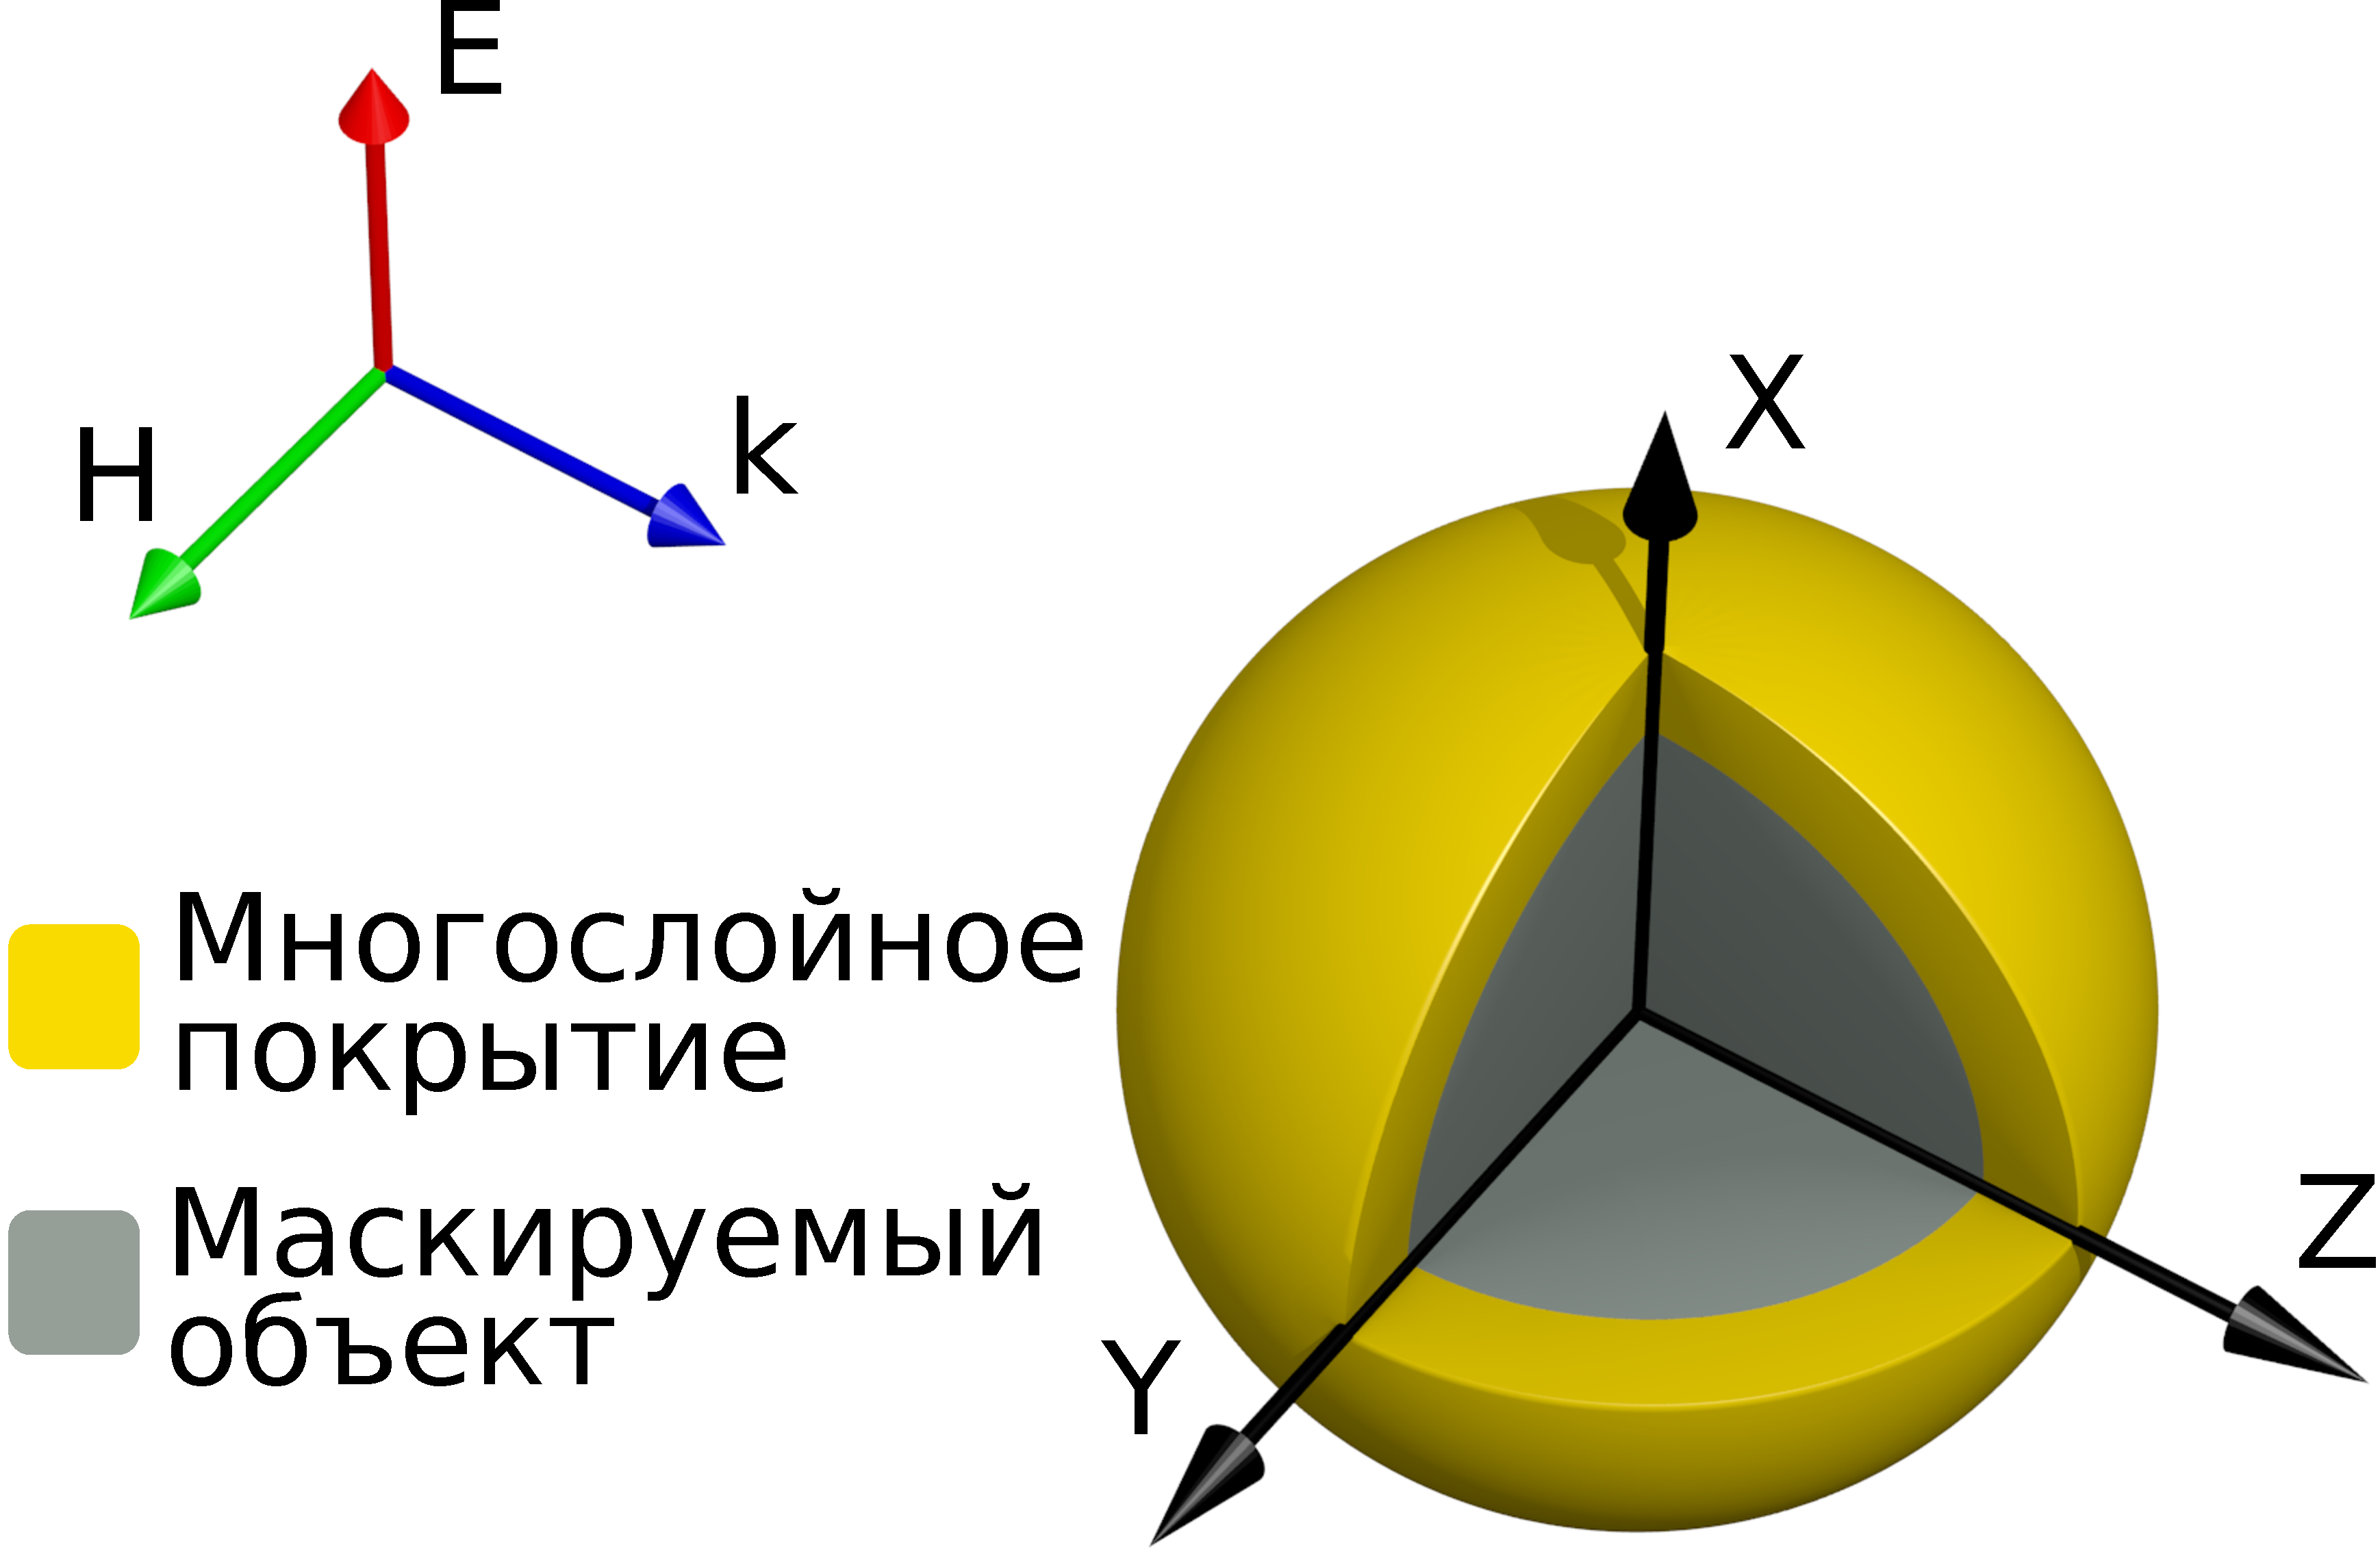
\includegraphics[width=0.8\linewidth]{model-view}    \\
    % \vspace{1em}\\
    \vspace{1em}
   \small \textit{Ladutenko et. al.},
   {J. Appl. Phys.}, vol. 116, pp. 184508  (\textbf{2014})
\end{center}
\end{frame}

\begin{frame}
  \frametitle{\normalsize Маскирующее диэлектрическое покрытие:}
  \small
  \begin{center}
  \hfill
  \begin{minipage}[ht]{0.48\linewidth}
    \centering{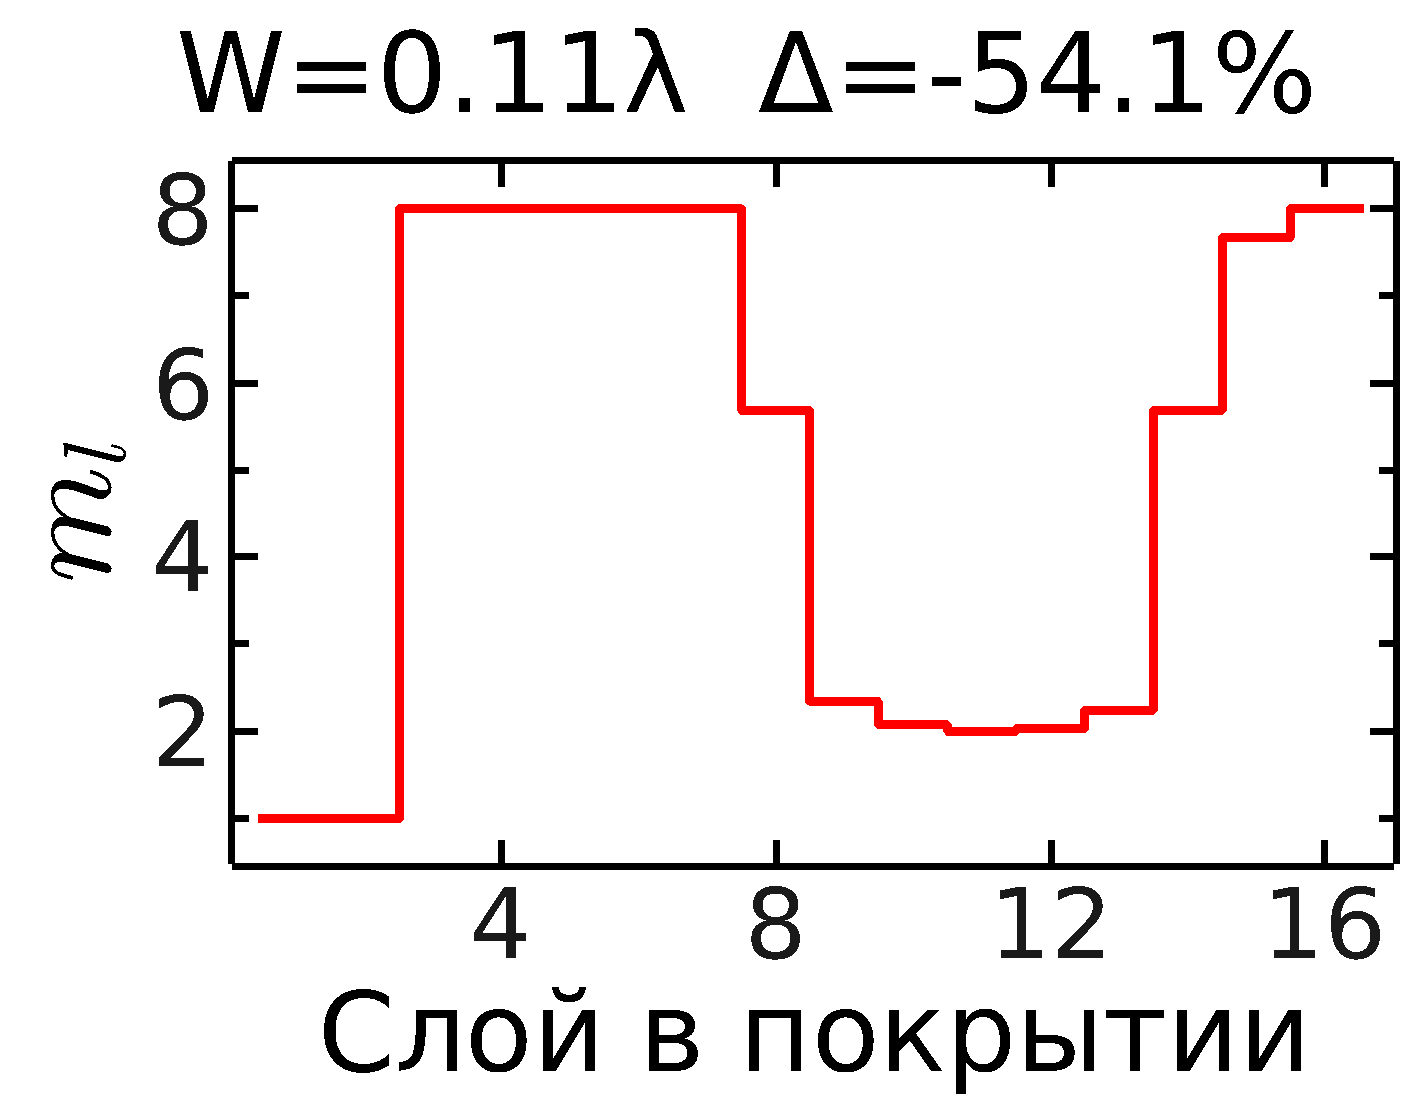
\includegraphics[width=0.95\linewidth]{w04-single-valley-index} \\ а)}
  \end{minipage}
  \hfill
  \begin{minipage}[ht]{0.48\linewidth}
    \centering{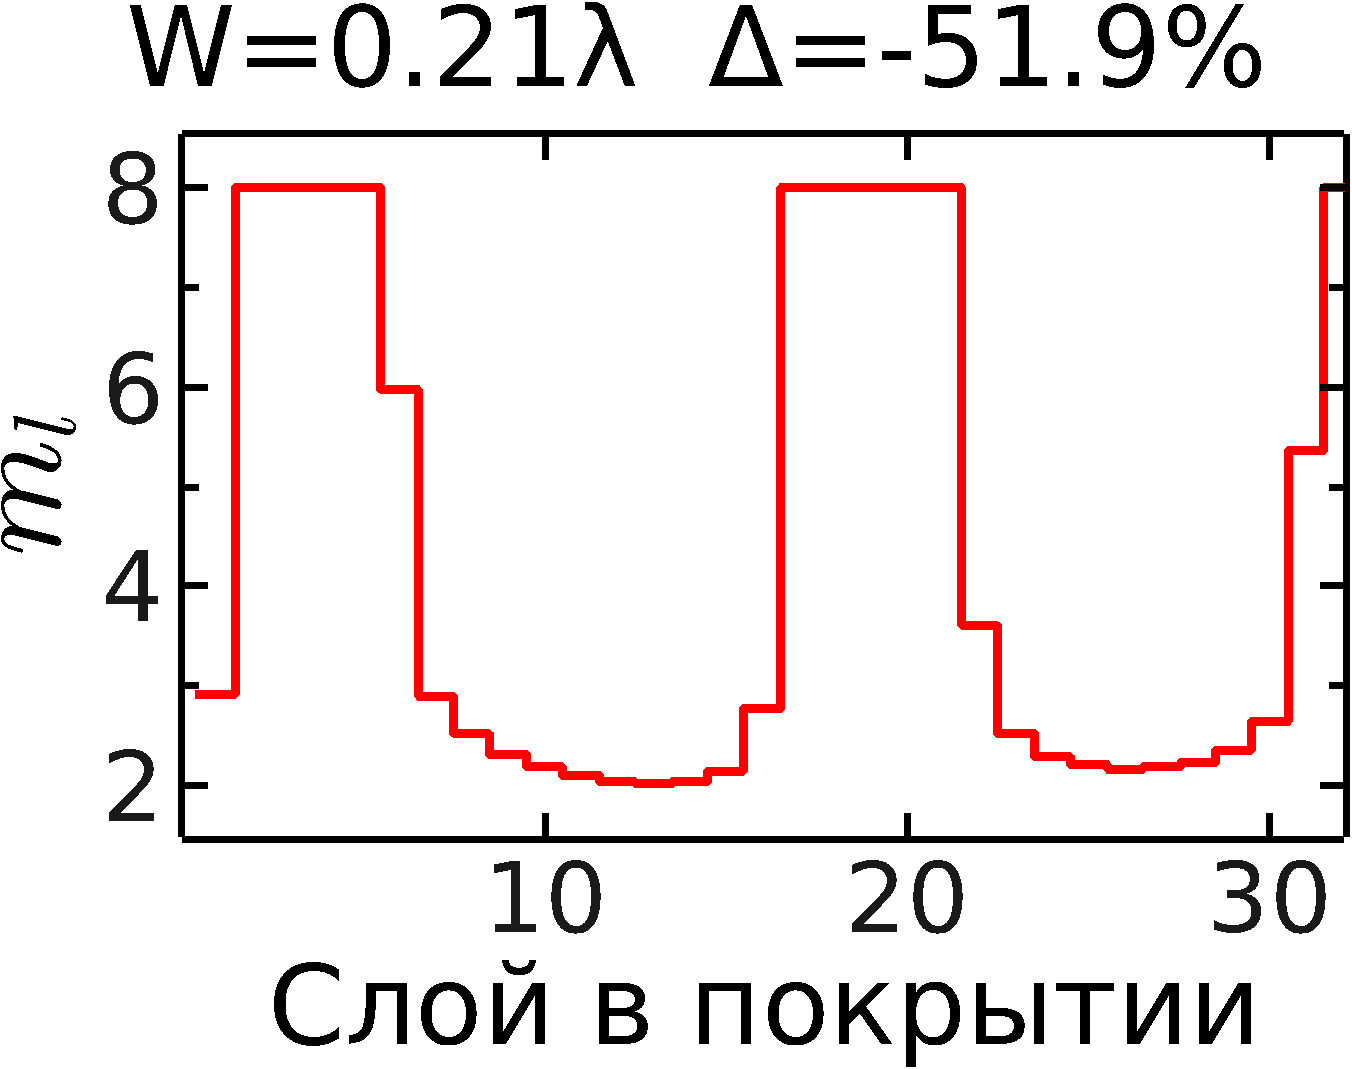
\includegraphics[width=0.95\linewidth]{w08-double-valley-index} \\ б)}
  \end{minipage}
  % \begin{minipage}[ht]{0.32\linewidth}
  %   \centering{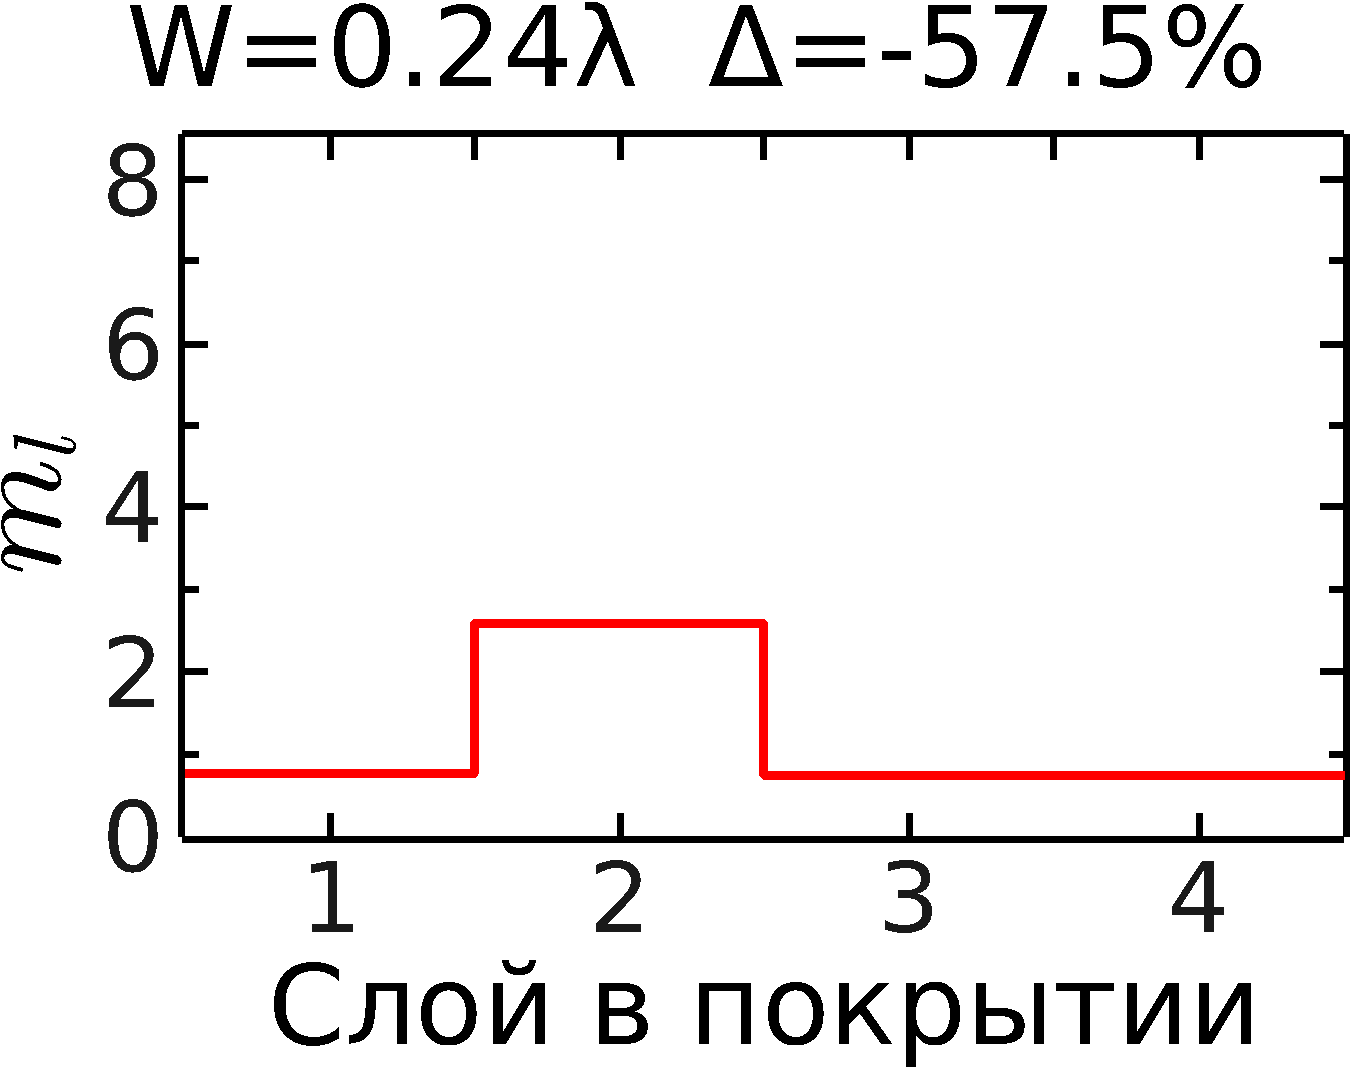
\includegraphics[width=0.95\linewidth]{index07-TO} \\ в)}
  % \end{minipage}
 Дизайны, обеспечивающие наилучшую маскировку мишени ${R_1 =
  0.75\lambda}$ при
    толщине покрытия,\\ равной (a)~$0.11\lambda$ и
    (б)~$0.21\lambda$.\\  Значение показателя преломления
    было ограничено\\ $n_{\mathrm{max}}=8$ и $n_{\mathrm{min}}=1$ 
\end{center}
\end{frame}


\begin{frame}
\begin{center}
\small
  \begin{minipage}[ht]{0.49\linewidth}
    \centering{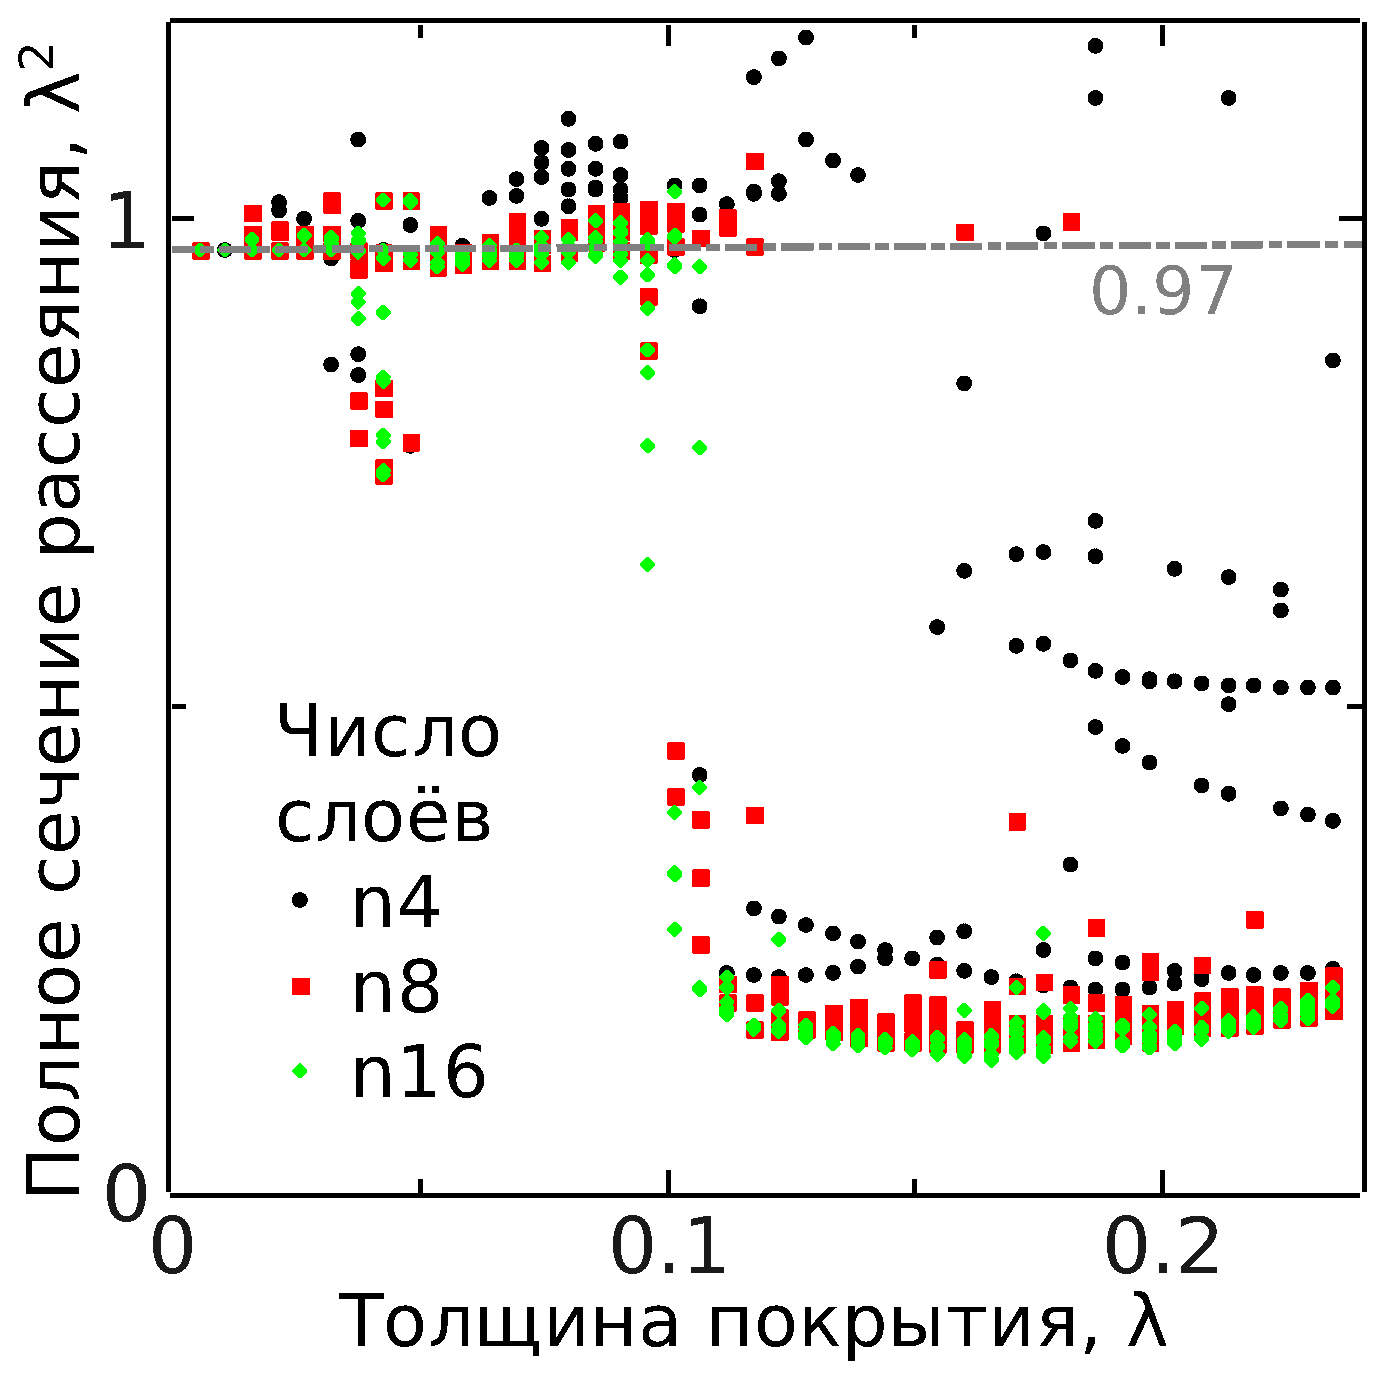
\includegraphics[width=0.99\linewidth]{rcs-overview-r14}\\a)}    
  \end{minipage}
  \begin{minipage}[ht]{0.49\linewidth}
    \centering{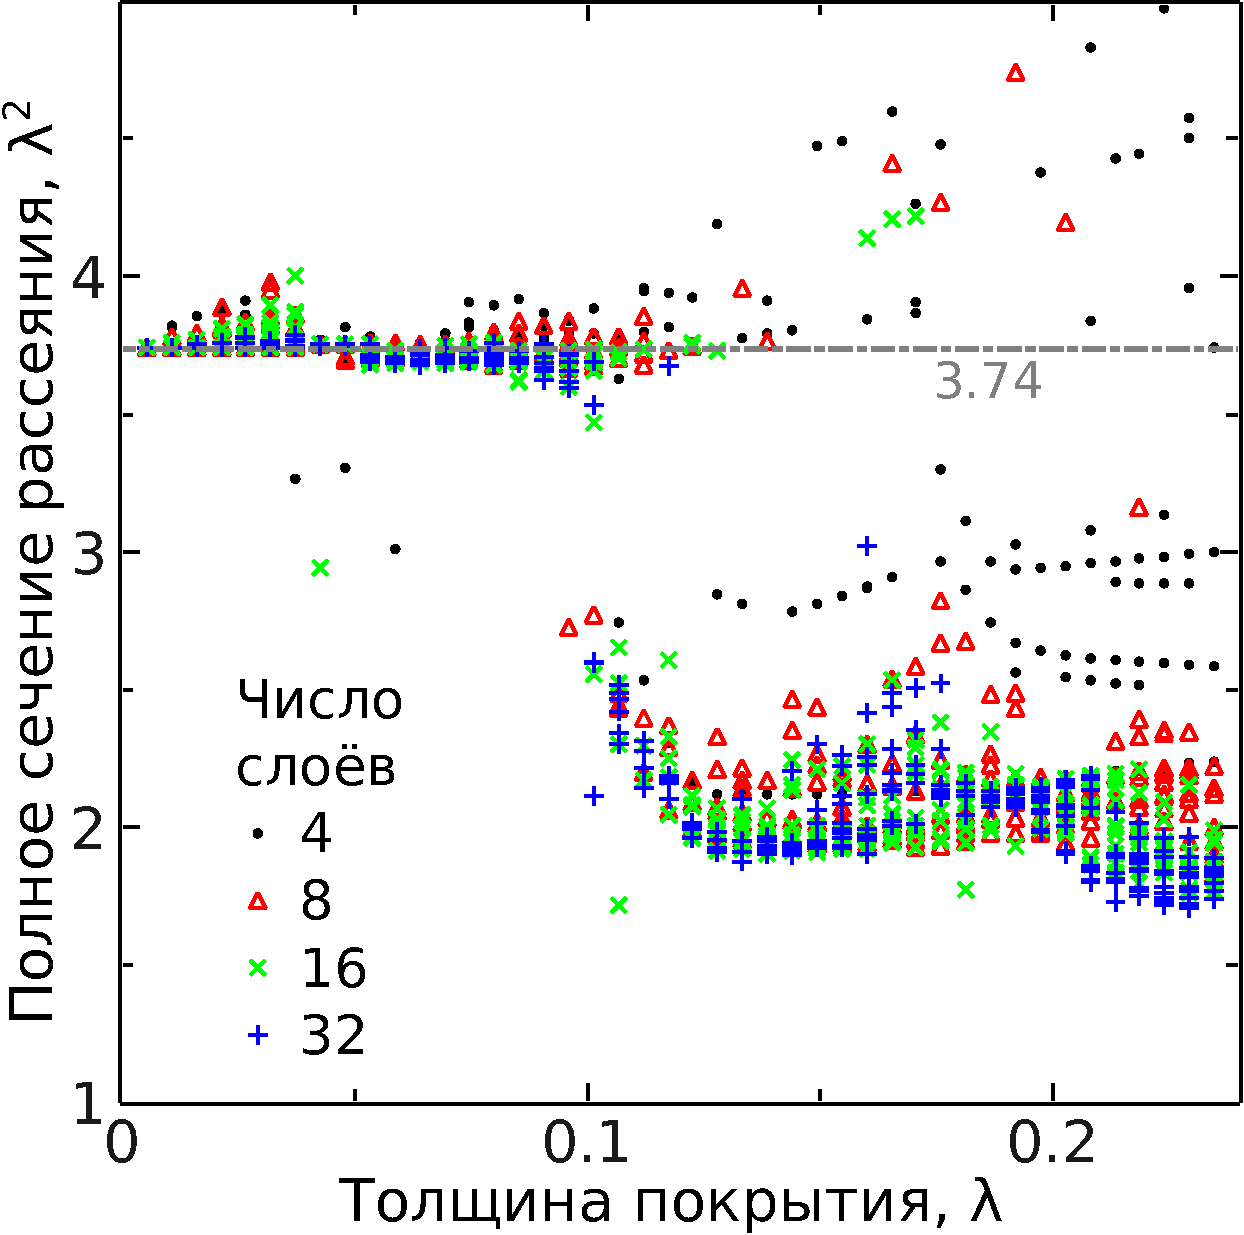
\includegraphics[width=0.99\linewidth]{rcs-overview}\\б)}
  \end{minipage}
  Результат оптимизации для мишени (a)~${R = 0.38\lambda}$ и
    (б)~${R = 0.75\lambda}$. Каждая отметка на графике
    соответствует одному дизайну, полученному в результате
    минимизации рассеяния. Типичное значение уменьшения TSCS
    составило приблизительно -85\% и -35\%
    соответственно.%
\end{center}
\end{frame}

\begin{frame}
%   \begin{center}
% \textbf{    Исследование рассеяния и поглощения электромагнитных волн
%     многослойными сферическими наночастицами.
% }  \end{center}
  \begin{center}
    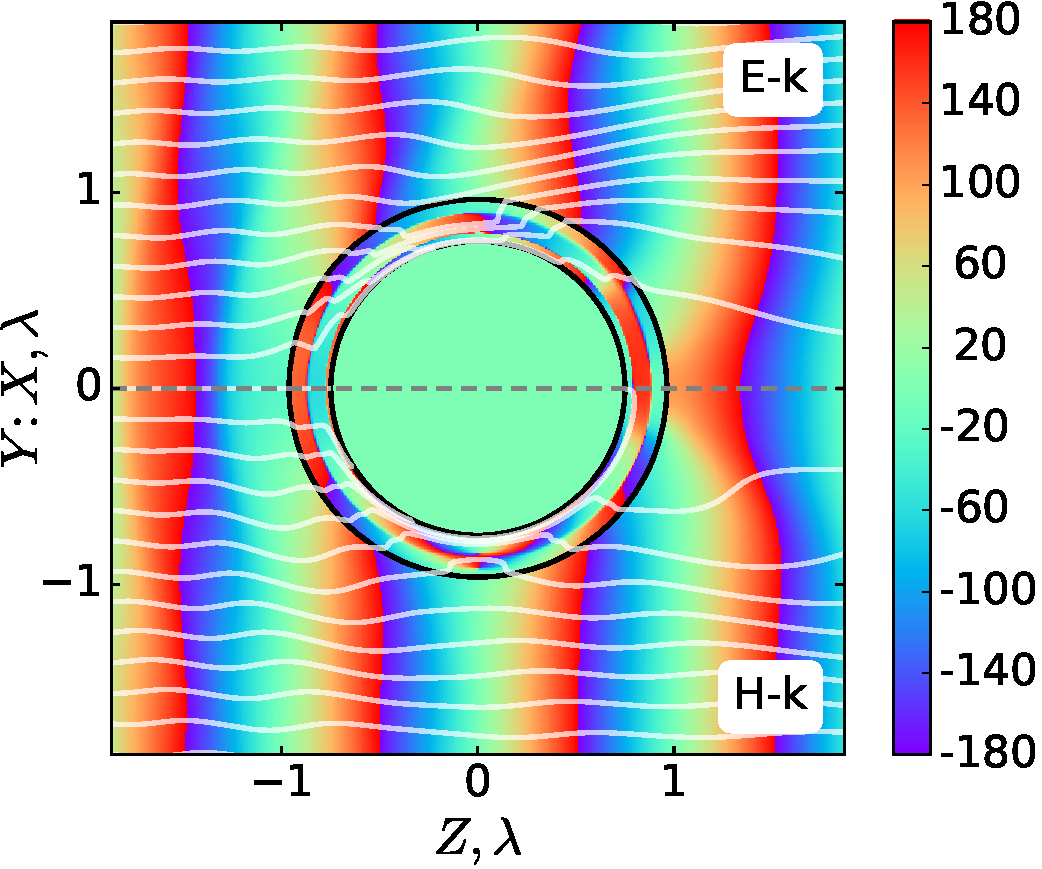
\includegraphics[width=0.8\linewidth]{PEC-index-dv-R4-XYZ-angleHy-rainbow}    \\
    % \vspace{1em}\\
    \vspace{1em} \small Дополнительный набег фазы магнитного поля при
    маскировке мишени ${R = 0.75\lambda}$ покрытием толщиной
    $0.21\lambda$.
\end{center}
\end{frame}

\begin{frame}
  \frametitle{Положение 2}
  \begin{center} Рассеяние на объекте из идеального проводника можно
    существенно уменьшить с помощью тонкого (по сравнению с длиной
    волны $\lambda$) многослойного покрытия, используя только
    изотропные диэлектрические материалы: для объектов диаметром
    $1.5\lambda$ в два раза, для диаметра $\lambda/1.5$ - в 6
    раз. Оптимальная толщина покрытия определяется доступным
    диапазоном применяемых материальных параметров.
  \end{center}
\end{frame}

\begin{frame}
\small
\begin{center}
  Рассмотрим оптимизацию маскирующего покрытия для частицы,
  находящейся в среде.\\
  \vspace{1em}
  Это эквивалентно случаю частицы в вакууме и
  использованию в покрытии материалов с ${\varepsilon<1}$.
\end{center}
\end{frame}

\begin{frame}
\begin{center}
\small
  \begin{minipage}[ht]{0.49\linewidth}
    \centering{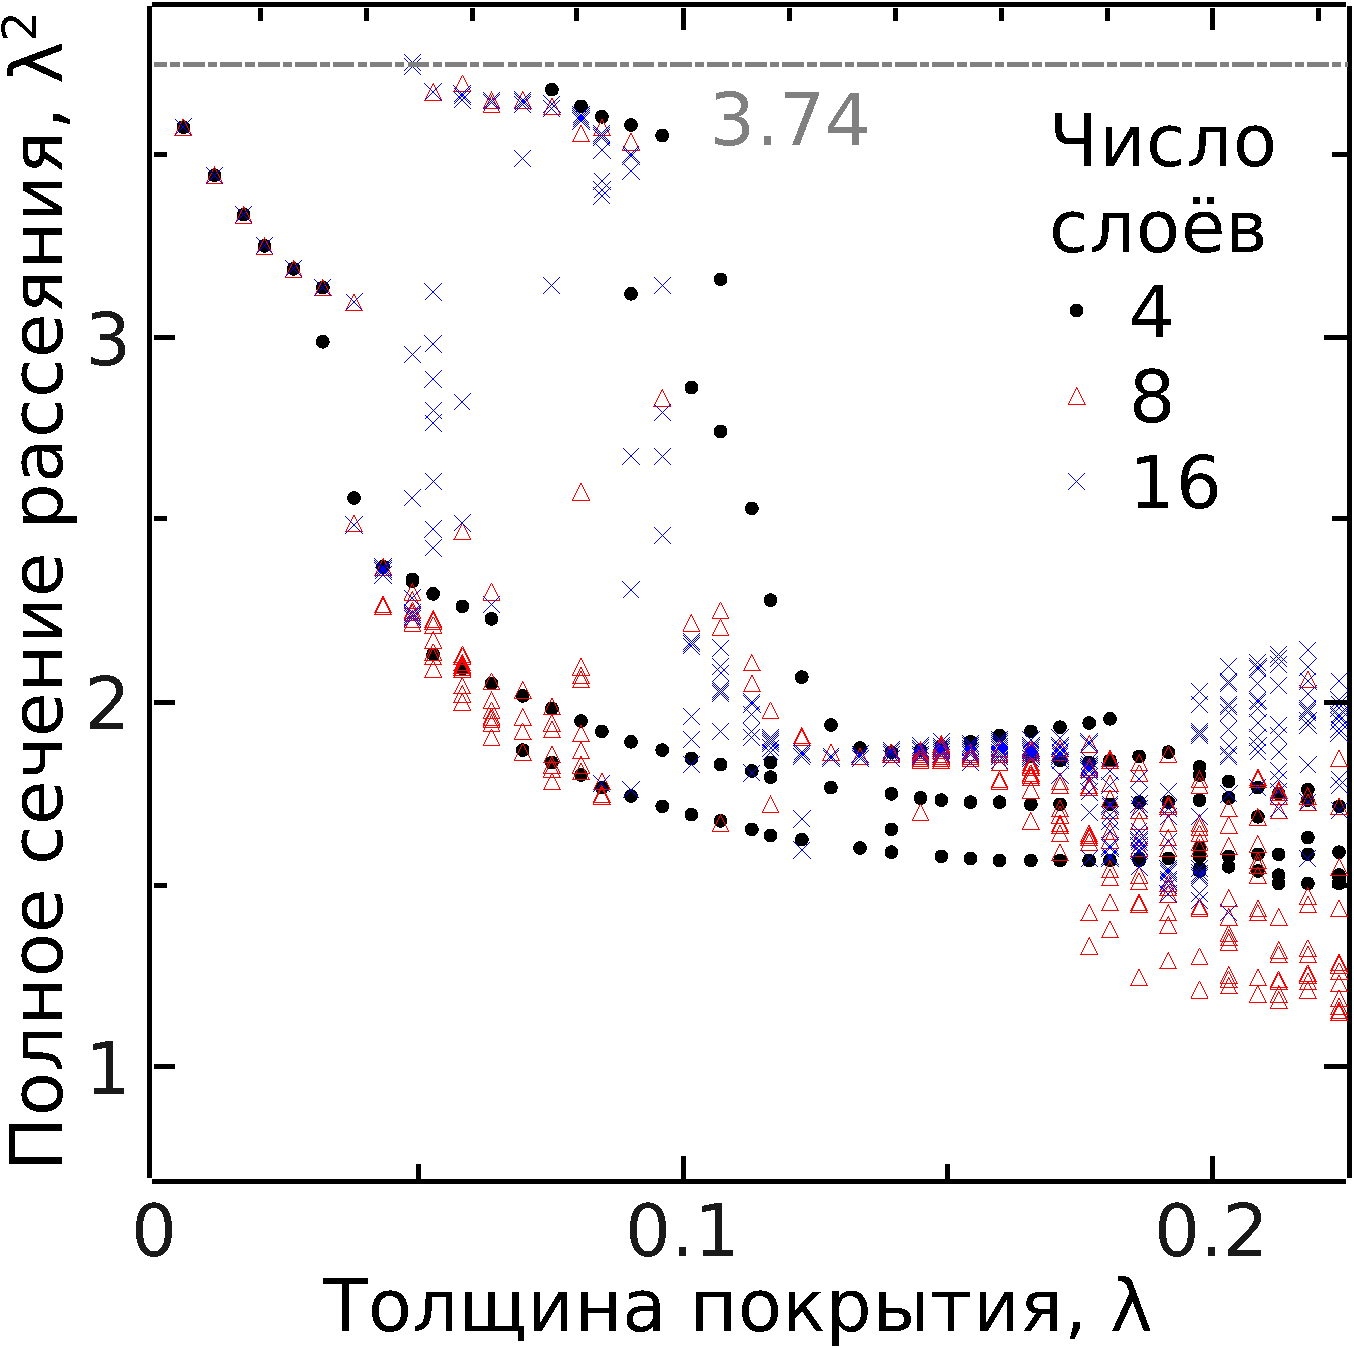
\includegraphics[width=0.99\linewidth]{rcs-overview-index07-color}\\a)}    
  \end{minipage}
  \begin{minipage}[ht]{0.49\linewidth}
    \centering{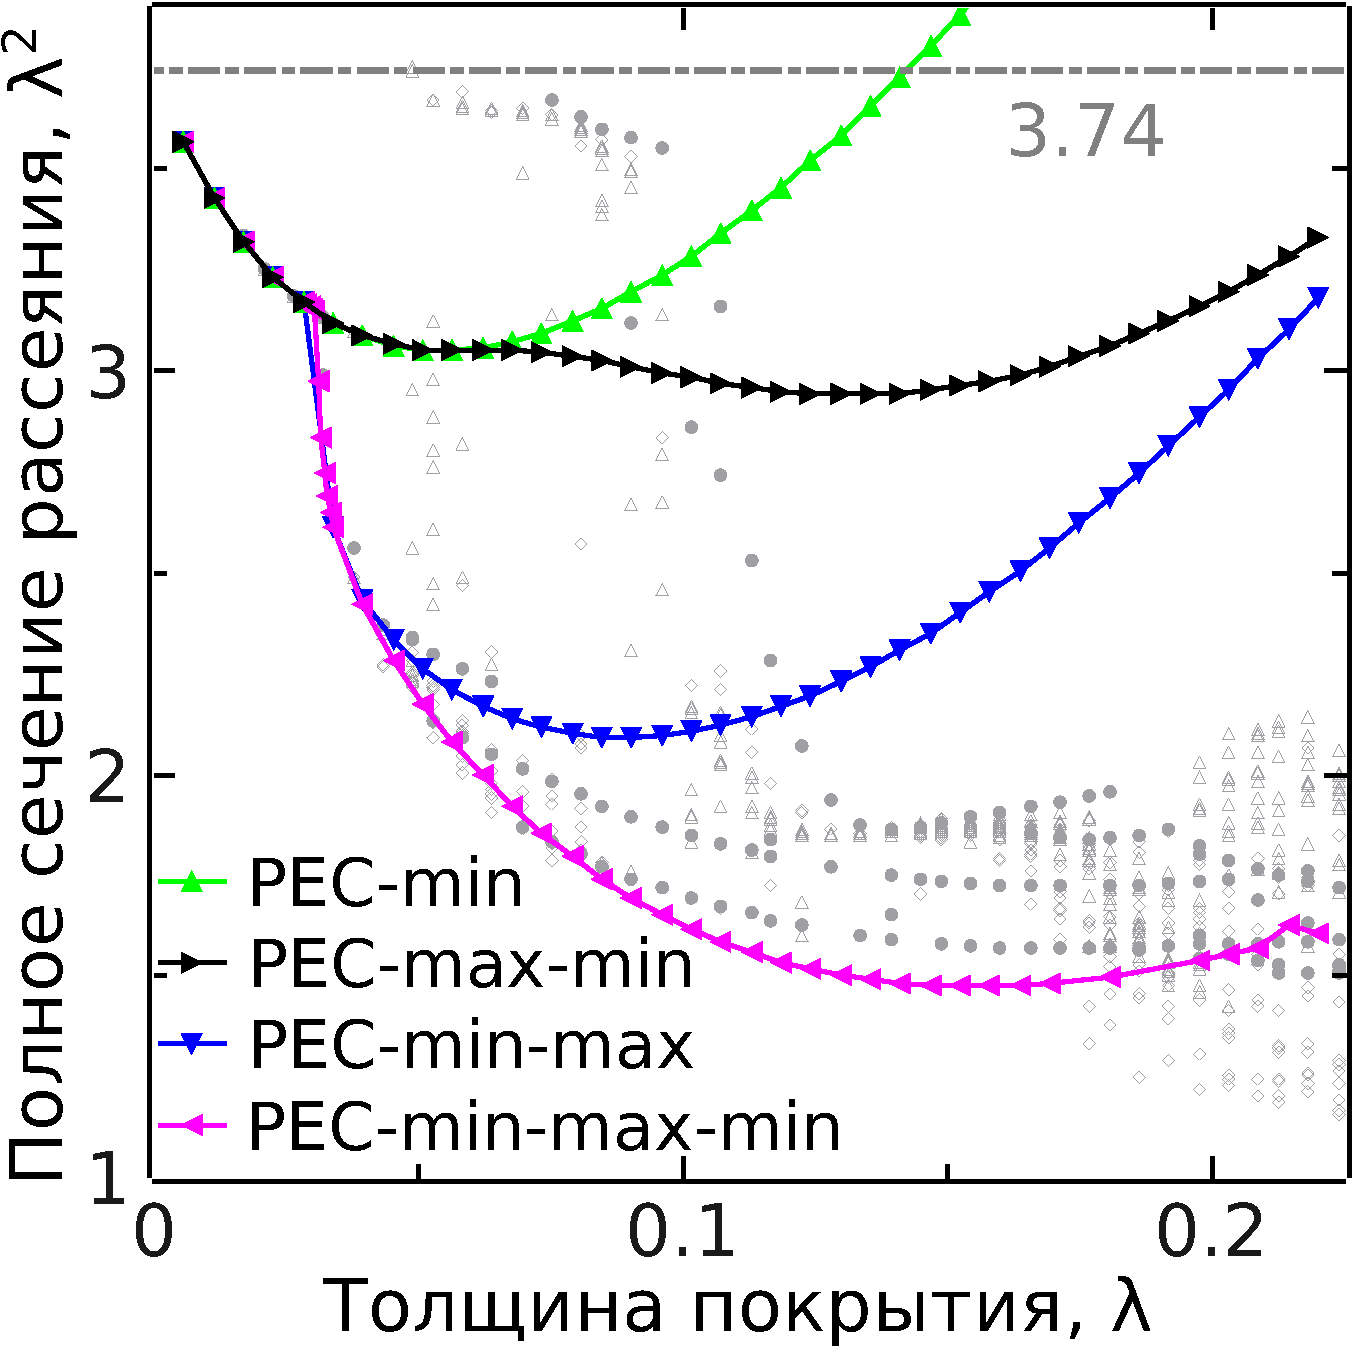
\includegraphics[width=0.99\linewidth]{rcs-overview-index07-DI}\\б)}
  \end{minipage}
  
  Результат оптимизации  для мишени ${R = 0.75\lambda}$ а) показателей преломления в каждом
    слое при его фиксированной толщине и б) толщины каждого слоя для
    покрытий с чередующимися слоями из большого $\varepsilon$ и
    ${\varepsilon<1}$.
1\end{center}
\end{frame}

\begin{frame}
\begin{center}
\small
  \begin{minipage}[ht]{0.55\linewidth}
    \centering{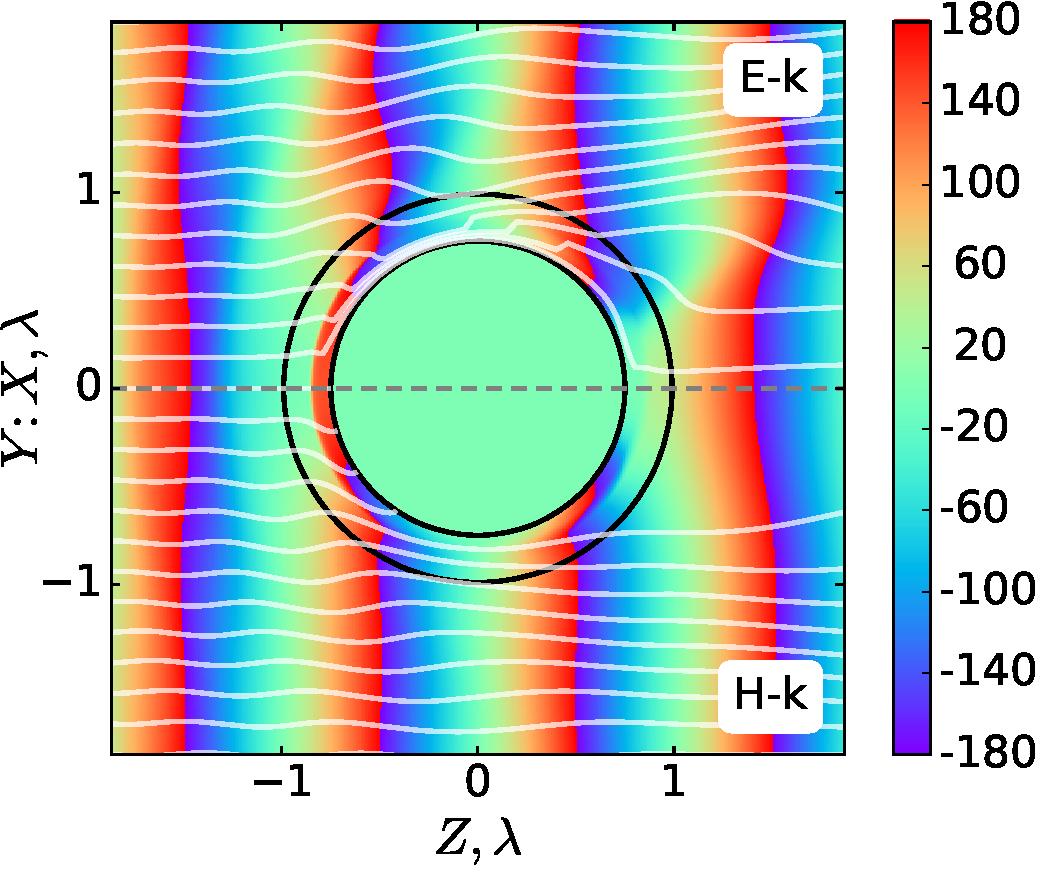
\includegraphics[width=0.99\linewidth]{PEC-index-in-glass-R4-XYZ-angleHy-rainbow}\\a)}    
  \end{minipage}
  \begin{minipage}[ht]{0.43\linewidth}
    \centering{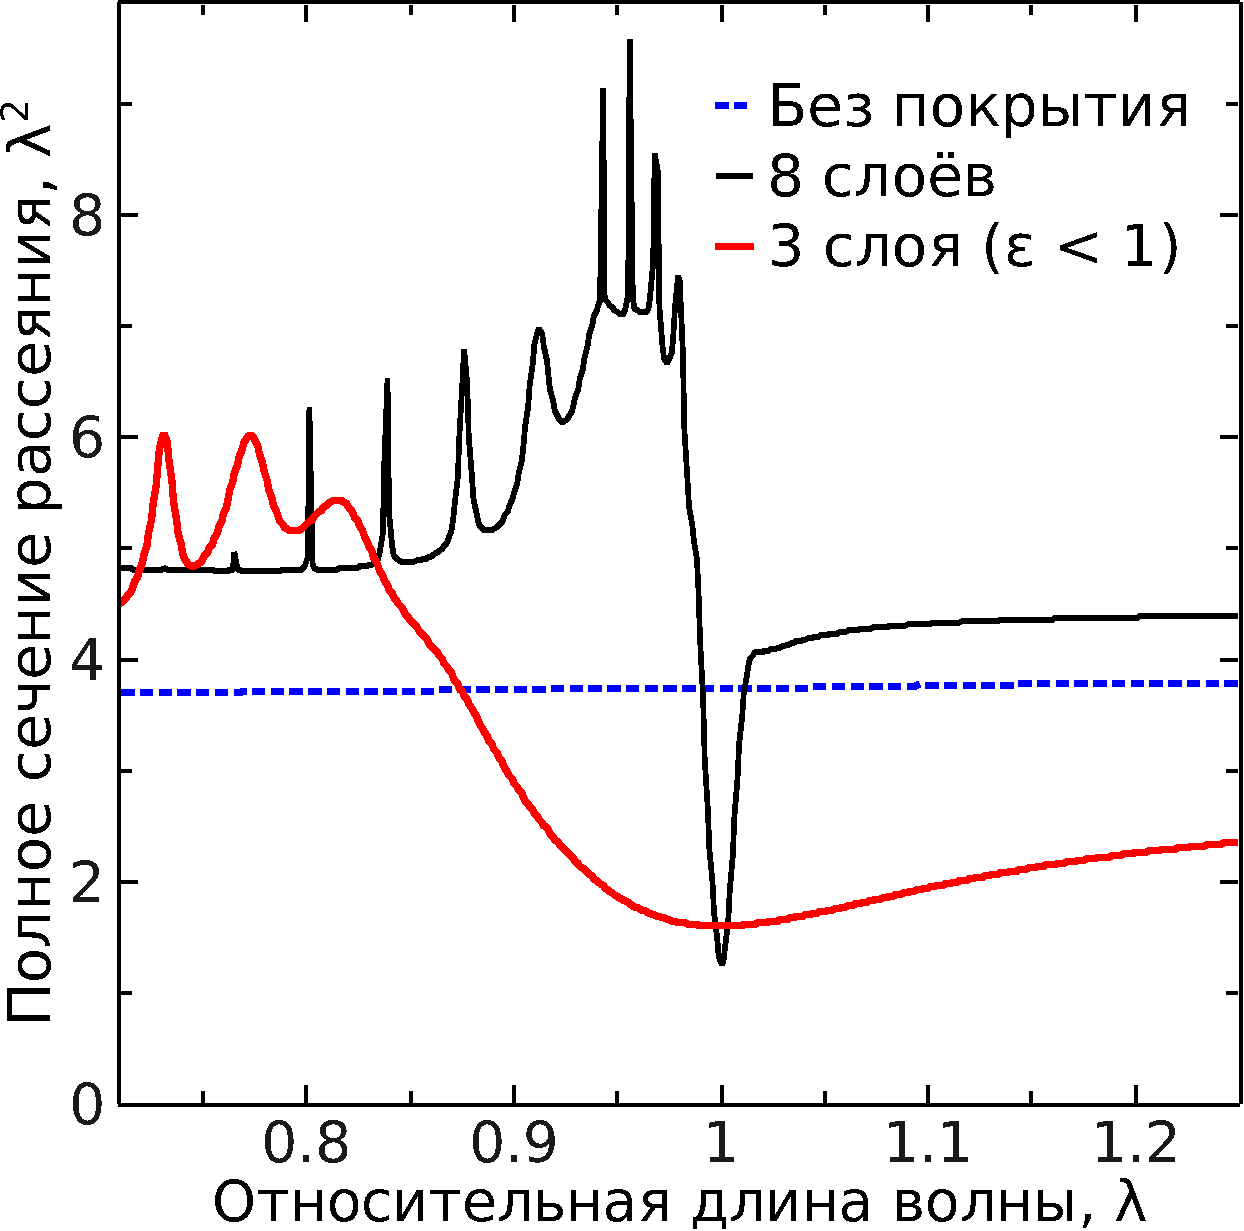
\includegraphics[width=0.99\linewidth]{index07-spectra}\\б)}
  \end{minipage}
  а) Фаза магнитного поля при маскировке мишени ${R = 0.75\lambda}$
  покрытием с ${\varepsilon<1}$. б) Спектры частицы без покрытия и с маскирующими
    покрытиями: из 8-ми слоёв диэлектрика и из 3-х слоёв с применением
    ${\varepsilon<1}$.
\end{center}
\end{frame}
\begin{frame}
  \frametitle{Положение 3}
  \begin{center}     При анализе покрытий из множества слоёв равной толщины
    была выявлена закономерность, позволяющая разрабатывать
    сферические покрытия из трёх слоёв различной толщины, а именно,
    для достижения аналогичной эффективности маскировки достаточно
    чередования двух материалов, один из которых обладает
    $\varepsilon<1$. 
  \end{center}
\end{frame}

\begin{frame}
  \frametitle{Поглощение света}
  \begin{center}
На примере структуры $Si/Ag/Si$:
  \end{center}
  \begin{center}
    \includegraphics[width=0.6\linewidth]{model3d}    \\
    % \vspace{1em}\\
  \scriptsize Рисунок из работы \textit{Ladutenko et al.}, Nanoscale, 7, 18897 (\textbf{2015})
\end{center}
\end{frame}

\begin{frame}
  \frametitle{Поглощение света}
  \small
  \begin{itemize}
  \item {\em Эффективность поглощения}
    $Q_{\rm abs}=C_{\rm abs}/\pi R^2$ 
  \item Фундаментальный предел поглощения одним мультиполем:
    $Q^{(n)}_{\rm abs\ max}=\frac{2n+1}{2q^2}$, где параметр размера
    $q=2\pi R/\lambda$, $n$ --- порядок моды в мультипольном разложении.\\
    M. I. Tribelsky, \textit{EPL} 94, 14004 (2011)

  \item Преодоление фундаментального предела возможно за счёт совмещения
    нескольких мультипольных резонансов.
  \end{itemize}

\end{frame}  

\begin{frame}
  \frametitle{Поглощение света}
  \small
  \begin{center}
    \includegraphics[width=0.6\linewidth]{fig1-crop}    \\
    % \vspace{1em}\\
    Результат оптимизации поглощения света трёхслойной наночастицей
    $Si/Ag/Si$ для длины волны $\lambda = 500$~нм. 
  \end{center}
\end{frame}  

\begin{frame}
  \frametitle{Поглощение света}
  \small
  \begin{center}
    \footnotesize
    \includegraphics[width=0.6\linewidth]{fig2-crop}    \\
    % \vspace{1em}\\
    Коэффициенты поглощения, где $\tilde{a}_1$ и
    $\tilde{a}_2$ относятся к электрическим, а $\tilde{b}_1$ и
    $\tilde{b}_2$ к магнитным диполю и квадруполю.
  \end{center}
\end{frame}  

\begin{frame}
  % \frametitle{Поглощение света}
  \small
  \begin{center}
    \footnotesize
    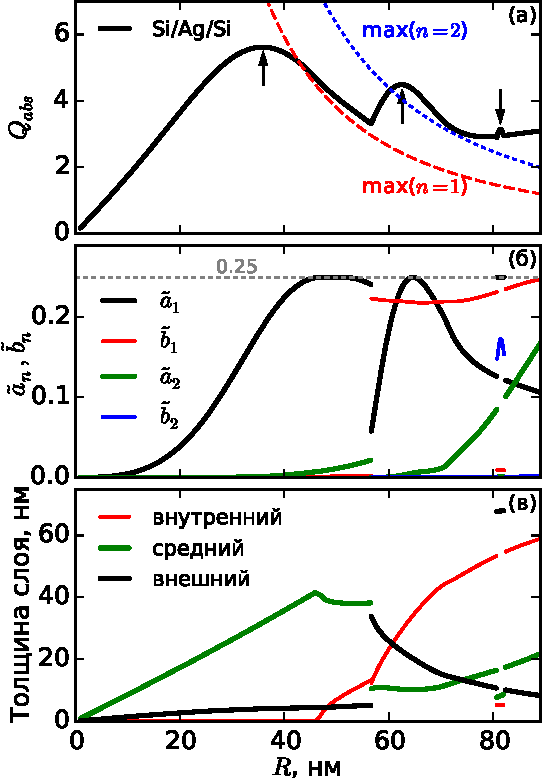
\includegraphics[width=0.57\linewidth]{2015-04-01-Qabs-SiAgSi-overview}   %  \\
    % % \vspace{1em}\\
    % Коэффициенты поглощения, где $\tilde{a}_1$ и
    % $\tilde{a}_2$ относятся к электрическим, а $\tilde{b}_1$ и
    % $\tilde{b}_2$ к магнитным диполю и квадруполю.
  \end{center}
\end{frame}  


\begin{frame}
  % \frametitle{Поглощение света}
  \small
  \begin{minipage}[ht]{0.49\linewidth}
    \centering{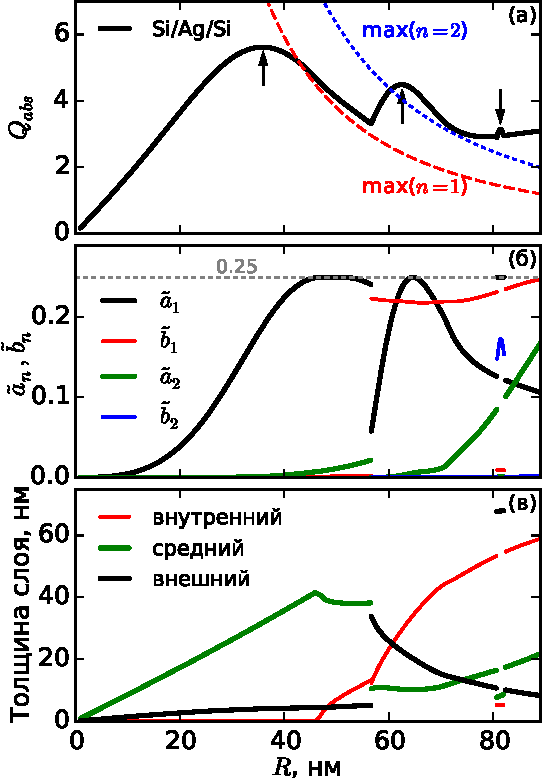
\includegraphics[height=1.35\linewidth]{2015-04-01-Qabs-SiAgSi-overview}}
  \end{minipage}
  \hfill
  \begin{minipage}[ht]{0.49\linewidth}
    \centering{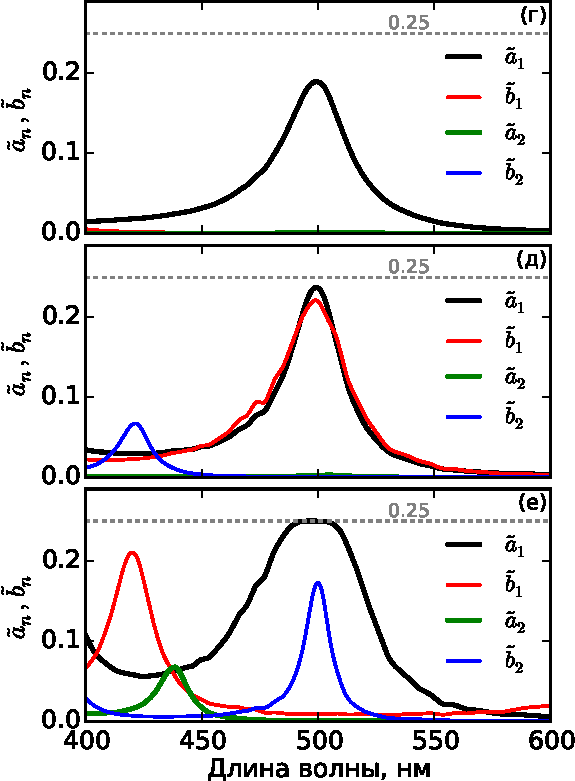
\includegraphics[height=1.35\linewidth]{2015-04-01-SiAgSi-ab-spectra4}}
  \end{minipage}
\end{frame}

\begin{frame}
  \frametitle{Положение 4}
  \begin{center}  На примере структуры $Si/Ag/Si$ показана возможность
    вырождения мультипольных резонансов в сферических трёхслойных
    наночастицах. Такое вырождение приводит к эффекту суперпоглощения,
    когда сечение поглощения оказывается больше, чем у однородной
    частицы того же размера из произвольного изотропного материала.
  \end{center}
\end{frame}
\begin{frame}
  \frametitle{Положение 5}
  \begin{center}
    Совместное применение теории Ми и стохастической оптимизации
    позволяет изучать предельно достижимые оптические свойства многослойных
    сферических наночастиц.
  \end{center}
\end{frame}

\begin{frame}
  \scriptsize 
  \textbf{Публикации автора по теме диссертации:}
  \begin{itemize}
  \item A1. Mie calculation of electromagnetic near-field for a multilayered sphere / K.
Ladutenko, U. Pal, A. Rivera, O. Peña-Rodríguez // Computer Physics Communications. — 2017. — Vol. 214. — P. 225–230.
\item A2. Superabsorption of light by nanoparticles / K. Ladutenko, P. Belov, O. Peña-
Rodríguez, A. Mirzaei, A. E. Miroshnichenko, I. V. Shadrivov // Nanoscale. —
2015. — Vol. 7, issue 45. — P. 18897–18901.
\item A3. Reduction of scattering using thin all-dielectric shells designed by stochastic
optimizer / K. Ladutenko, O. Peña-Rodríguez, I. Melchakova, I. Yagupov, P.
Belov // Journal of Applied Physics. — 2014. — Vol. 116, no. 18. —
P. 184508.
\item A4. Markovich D., Ladutenko K., Belov P. Performance of FDTD method CPU implementations for simulation of electromagnetic processes // Progress in Electromagnetics Research. — 2013. — Vol. 139. — P. 655–670.
\item A5. Ладутенко К. С., Белов П. А. Моделирование интегральных схем нанофотоники: метод FDTD // Наносистемы: физика, химия, математика. —
2012. — Т. 3. — С. 42—61.
  \end{itemize}
\end{frame}

\begin{frame}
  \scriptsize 
  \textbf{Публикации автора по теме диссертации:}
  \begin{itemize}
  \item A6. Beyond superabsorption: how to design efficient absorption of light by
nanoparticles / K. Ladutenko, P. Belov, O. Peña-Rodríguez, A. Mirzaei,
A. Miroshnichenko, I. Shadrivov // Metanano. Book of abstracts. — 2016. —
P. 14.
\item 
A7. Efficient absorption of light by nanoparticles designed by a stochastic optimizer / K. Ladutenko, P. Belov, O. Peña-Rodríguez, A. Mirzaei, A. Miroshnichenko, I. Shadrivov // Days on Diffraction. Book of abstracts. — 2016. —
P. 195.
\item A8. Sphere cloaking using thin all-dielectric multilayer coatings designed by
stochastic optimizer / K. Ladutenko, O. Peña-Rodríguez, I. Melchakova, I.
Yagupov, P. Belov // Days on Diffraction. Book of abstracts. — 2014. —
P. 117.
\item A9. Разработка тонких многослойных диэлектрических маскирующих покрытий с помощью стохастического оптимизатора / К. Ладутенко, O. P.
Rodríguez, И. Мельчакова, И. Ягупов, П. Белов // Электроника и
микроэлектроника СВЧ. Сборник тезисов. — 2014. — С. 285.
\item 
A10. К.C. Ладутенко Реализация алгоритма стохастической оптимизации
методом дифференциальной эволюции для численного исследования
металло-диэлектрических наноструктур и метаматериалов // бюллетень
Федеральной службы по интеллектуальной собственности (Роспатент)
«Программы для ЭВМ. Базы данных. Топологии интегральных микро-
схем». — 20.02.2014. — RU 2014611568
\end{itemize}
\end{frame}



\begin{frame}
  \frametitle{Личный вклад}
  \small
      \begin{center}
  \begin{itemize}
  \item Все результаты данной диссертационной работы получены автором
    лично, их анализ проводился при его непосредственном участии.
  \item Автор самостоятельно провёл все работы, связанные с
    программированием алгоритма стохастической оптимизации.
  \item Программа Scattnlay, используемая для расчётов по теории Ми,
    была полностью переработана автором диссертации совместно с
    автором оригинальной программы Ovidio Pe\~{n}a-Rodr\'{i}guez
    (Политехнический университет Мадрида, Испания).
  \end{itemize}
\end{center}
\end{frame}

\begin{frame} 
\begin{center}
Спасибо за внимание!
\end{center}
\end{frame}

\end{document} 